\chapter{Perancangan}
\label{chap:perancangan}

Bab ini membahas perancangan aplikasi desktop pemeriksa tautan rusak pada situs web berdasarkan hasil analisis yang telah dilakukan pada Bab~\ref{chap:analisis}. Perancangan mencakup rancangan kelas, perancangan alur dan perancangan antarmuka. Dengan adanya perancangan ini, implementasi dapat dilakukan secara lebih terarah dan sesuai dengan kebutuhan yang telah ditentukan.


\section{Perancangan Kelas}
\label{sec:04-perancangan-kelas}

Struktur kelas pada aplikasi \textit{Broken Link Checker} dibagi ke dalam tiga \textit{package} utama, yaitu \texttt{Web Crawling}, \texttt{URL Fetcher}, dan \texttt{GUI Manager}. \textit{Package} \texttt{Web Crawling} berisi kelas-kelas inti yang mengatur proses \textit{crawling}, pengelolaan \textit{frontier}, serta representasi tautan. \textit{Package} \texttt{URL Fetcher} menyediakan mekanisme untuk mengambil konten dari situs web menggunakan pustaka eksternal seperti Jsoup dan \texttt{HttpClient}. Sementara itu, \textit{package} \texttt{GUI Manager} menangani pengelolaan antarmuka pengguna dengan JavaFX, termasuk kontrol proses pemeriksaan dan penyajian hasil. Diagram kelas untuk aplikasi ini dapat dilihat pada Gambar~\ref{fig:class-diagram}.

Penjelasan setiap kelas pada diagram adalah sebagai berikut:

\begin{enumerate}
    \item \textbf{Kelas Link}\\  
    Kelas \texttt{Link} merupakan kelas dasar yang merepresentasikan sebuah tautan dalam sistem. Kelas ini menjadi induk bagi \texttt{WebpageLink} dan \texttt{BrokenLink}, sehingga relasinya berupa pewarisan.
    \begin{itemize}
        \item \texttt{url} : Atribut ini bertipe data \textit{String} dan digunakan untuk menyimpan alamat dari tautan yang diperiksa.
        \item \texttt{statusCode} : Atribut ini bertipe data \textit{int} dan berfungsi untuk menyimpan kode status HTTP hasil pemeriksaan tautan.
        \item \texttt{accessTime} : Atribut ini bertipe data \textit{Instant} dan merekam waktu terakhir kali tautan tersebut diakses.
    \end{itemize}

    \item \textbf{Kelas WebpageLink}\\
    Kelas \texttt{WebpageLink} merepresentasikan tautan yang termasuk dalam kategori halaman web dengan \textit{host} yang sama seperti URL awal. Kelas ini mewarisi \texttt{Link} dan memiliki relasi \textit{many-to-many} dengan \texttt{BrokenLink}.
    \begin{itemize}
        \item \texttt{brokenLinks} : Atribut ini bertipe data \textit{Map<BrokenLink, String>} dan digunakan untuk menyimpan daftar tautan rusak yang ditemukan di halaman beserta informasi anchor text-nya.
    \end{itemize}

    \item \textbf{Kelas BrokenLink}\\
    Kelas \texttt{BrokenLink} digunakan untuk menyimpan data tautan yang gagal diakses atau menghasilkan status \textit{error}. Kelas ini mewarisi \texttt{Link} dan memiliki relasi \textit{many-to-many} dengan \texttt{WebpageLink}.
    \begin{itemize}
        \item \texttt{webpageLinks} : Atribut ini bertipe data \textit{Map<WebpageLink, String>} dan digunakan untuk mencatat daftar halaman tempat tautan rusak tersebut ditemukan beserta lokasi anchor text-nya.
    \end{itemize}

    \item \textbf{Kelas Crawler}\\
    Kelas \texttt{Crawler} merupakan inti dari proses \textit{web crawling} dan bertanggung jawab mengelola antrean URL, melakukan pengambilan halaman, serta memeriksa status tautan. Kelas ini berhubungan langsung dengan \texttt{Frontier}, \texttt{WebpageLink}, dan \texttt{BrokenLink}, serta memiliki dependensi terhadap \texttt{Jsoup} dan \texttt{HttpClient}.
    \begin{itemize}

        \item \texttt{rootHost} : Atribut ini bertipe data \textit{String} dan digunakan untuk menyimpan host dari URL awal (seed URL).
        
        \item \texttt{frontier} : Atribut ini bertipe data \textit{Frontier} dan berfungsi sebagai antrean URL yang akan diproses.
        
        \item \texttt{repository} : Atribut ini bertipe data \textit{Set<String>} dan digunakan untuk menyimpan daftar URL yang sudah pernah dikunjungi agar tidak diperiksa dua kali.
        
        \item \texttt{USER\_AGENT} : Atribut statis ini bertipe data \textit{String} dan digunakan untuk mendefinisikan identitas permintaan HTTP yang dikirim oleh aplikasi.
        
        \item \texttt{TIMEOUT} : Atribut statis ini bertipe data \textit{int} dan menentukan batas waktu maksimum koneksi HTTP.
        
        \item \texttt{HTTP\_CLIENT} : Atribut statis ini bertipe data \textit{HttpClient} dan digunakan sebagai klien bawaan Java untuk mengirim permintaan HTTP.

        \item \texttt{Crawler} : Metode ini merupakan konstruktor yang menerima parameter \texttt{seedUrl} bertipe data \textit{String} dan digunakan untuk menginisialisasi proses \textit{crawling}.
        
        \item \texttt{startCrawling} : Metode ini menerima parameter \texttt{streamBrokenLink} bertipe \textit{Consumer<BrokenLink>} dan tidak mengembalikan nilai. Metode ini berfungsi untuk memulai proses \textit{crawling} dan mengirim hasilnya secara \textit{streaming}.
        
        \item \texttt{extractLinks} : Metode ini menerima parameter \texttt{doc} bertipe \textit{Document} dan mengembalikan daftar objek \texttt{BrokenLink}. Metode ini digunakan untuk mengekstrak seluruh tautan dari halaman HTML yang diambil.
        
        \item \texttt{normalizeUrl} : Metode ini menerima parameter \texttt{url} bertipe \textit{String} dan mengembalikan hasil normalisasi dalam bentuk \textit{String}. Metode ini digunakan untuk memastikan URL dalam format yang konsisten.
        
        \item \texttt{fetchUrl} : Metode ini menerima parameter \texttt{url} bertipe \textit{String} dan mengembalikan nilai \textit{int} yang merupakan kode status HTTP hasil pemeriksaan. Metode ini berfungsi untuk melakukan pemeriksaan tautan eksternal atau tautan umum menggunakan Java \texttt{HttpClient}.
        
        \item \texttt{isPotentialWebpage} : Metode ini menerima parameter \texttt{url} bertipe \textit{String} dan mengembalikan nilai \textit{boolean}. Metode ini digunakan untuk menentukan apakah suatu URL berpotensi merupakan halaman web.
    
    \end{itemize}

    \item \textbf{Kelas Frontier}\\
    Kelas \texttt{Frontier} berfungsi sebagai struktur data antrean (\textit{queue}) yang menyimpan URL yang akan diproses berikutnya. Kelas ini berelasi erat dengan \texttt{Crawler} yang mengelola antrean selama proses \textit{crawling} berlangsung.
    \begin{itemize}
        \item \texttt{urls} : Atribut ini bertipe data \textit{Queue<String>} dan digunakan untuk menampung daftar URL yang menunggu diproses.
        \item \texttt{enqueue} : Metode ini menerima parameter \texttt{url} bertipe \textit{String} dan berfungsi untuk menambahkan URL baru ke dalam antrean.
        \item \texttt{dequeue} : Metode ini tidak menerima parameter dan mengembalikan nilai \textit{String} berupa URL paling depan dari antrean.
        \item \texttt{isEmpty} : Metode ini tidak menerima parameter dan mengembalikan nilai \textit{boolean} untuk menunjukkan apakah antrean kosong atau tidak.
    \end{itemize}

    \item \textbf{Kelas Jsoup dan HttpClient}\\
    Kedua kelas ini merupakan representasi dari pustaka eksternal yang digunakan untuk melakukan pengambilan data web dan digunakan sebagai dependensi oleh kelas \texttt{Crawler}.
    \begin{itemize}
        \item \texttt{Jsoup} : Kelas ini digunakan untuk mengakses dan mengurai dokumen HTML dari halaman same-host dengan memanfaatkan parser HTML toleran kesalahan.
        \item \texttt{HttpClient} : Kelas ini digunakan untuk melakukan permintaan \texttt{HEAD} atau \texttt{GET} terhadap tautan umum atau eksternal untuk memeriksa status HTTP-nya.
    \end{itemize}

    \item \textbf{Kelas Controller}  
    Kelas \texttt{Controller} berfungsi sebagai penghubung antara logika aplikasi dengan antarmuka pengguna yang dibangun menggunakan JavaFX. Kelas ini berinteraksi dengan \texttt{Crawler} untuk menginisiasi dan menerima hasil proses pemeriksaan tautan.
    \begin{itemize}
        
        \item \texttt{seedUrlField} : Atribut ini bertipe \textit{TextField} dan digunakan untuk menampung input URL dari pengguna.
            
        \item \texttt{progressLabel} : Atribut ini bertipe \textit{Label} dan menampilkan status kemajuan proses pemeriksaan.
            
        \item \texttt{totalLinksLabel} : Atribut ini bertipe \textit{Label} dan menampilkan jumlah total tautan yang diperiksa.
        
        \item \texttt{webpagesLabel} : Atribut ini bertipe \textit{Label} dan menampilkan jumlah halaman yang berhasil di-crawl.
        
        \item \texttt{brokenLinksLabel} : Atribut ini bertipe \textit{Label} dan menampilkan jumlah tautan rusak yang ditemukan.
        
        \item \texttt{resultsTable} : Atribut ini bertipe \textit{TableView<BrokenLink>} dan menampilkan hasil daftar tautan rusak.
        
        \item \texttt{statusColumn} : Atribut ini bertipe \textit{TableColumn<BrokenLink, String>} dan digunakan untuk menampilkan kolom status pada tabel hasil.
        
        \item \texttt{urlColumn} : Atribut ini bertipe \textit{TableColumn<BrokenLink, String>} dan digunakan untuk menampilkan kolom URL tautan pada tabel hasil.
        
        \item \texttt{initialize} : Metode ini tidak menerima parameter dan berfungsi untuk melakukan inisialisasi awal saat antarmuka dimuat.
        
        \item \texttt{onStartClick} : Metode ini tidak menerima parameter dan digunakan untuk menangani event ketika pengguna menekan tombol \textit{Start}, kemudian memulai proses pemeriksaan tautan.
        
        \item \texttt{onStopClick} : Metode ini tidak menerima parameter dan digunakan untuk menghentikan proses pemeriksaan yang sedang berlangsung.
        
        \item \texttt{onExportClick} : Metode ini tidak menerima parameter dan digunakan untuk mengekspor hasil pemeriksaan ke dalam berkas Excel.
    \end{itemize}

    \item \textbf{Kelas Application}\\
    Kelas \texttt{Application} merupakan titik masuk (\textit{entry point}) dari aplikasi JavaFX. Kelas ini berhubungan dengan \texttt{Controller} untuk memuat dan menginisialisasi GUI.
    \begin{itemize}
        \item \texttt{main} : Metode ini tidak menerima parameter dan digunakan untuk menjalankan aplikasi.
        \item \texttt{start} : Metode ini menerima parameter \texttt{stage} bertipe \textit{Stage} dan berfungsi untuk memuat serta menampilkan antarmuka pengguna utama.
    \end{itemize}

    \item \textbf{Kelas HttpStatus}\\
    Kelas \texttt{HttpStatus} berfungsi sebagai kelas utilitas yang memetakan kode status HTTP ke \textit{reason phrase}. Kelas ini digunakan oleh \texttt{Controller} untuk menampilkan hasil status HTTP pada GUI.
    \begin{itemize}
        \item \texttt{STATUS\_MAP} : Atribut ini bertipe \textit{Map<Integer, String>} dan digunakan untuk menyimpan pasangan antara kode status HTTP dengan keterangan resminya.
        \item \texttt{getStatus} : Metode ini menerima parameter \texttt{statusCode} bertipe \textit{int} dan mengembalikan nilai \textit{String} berupa keterangan lengkap dari kode status tersebut.
    \end{itemize}
\end{enumerate}

\begin{figure}[H]
    \centering
    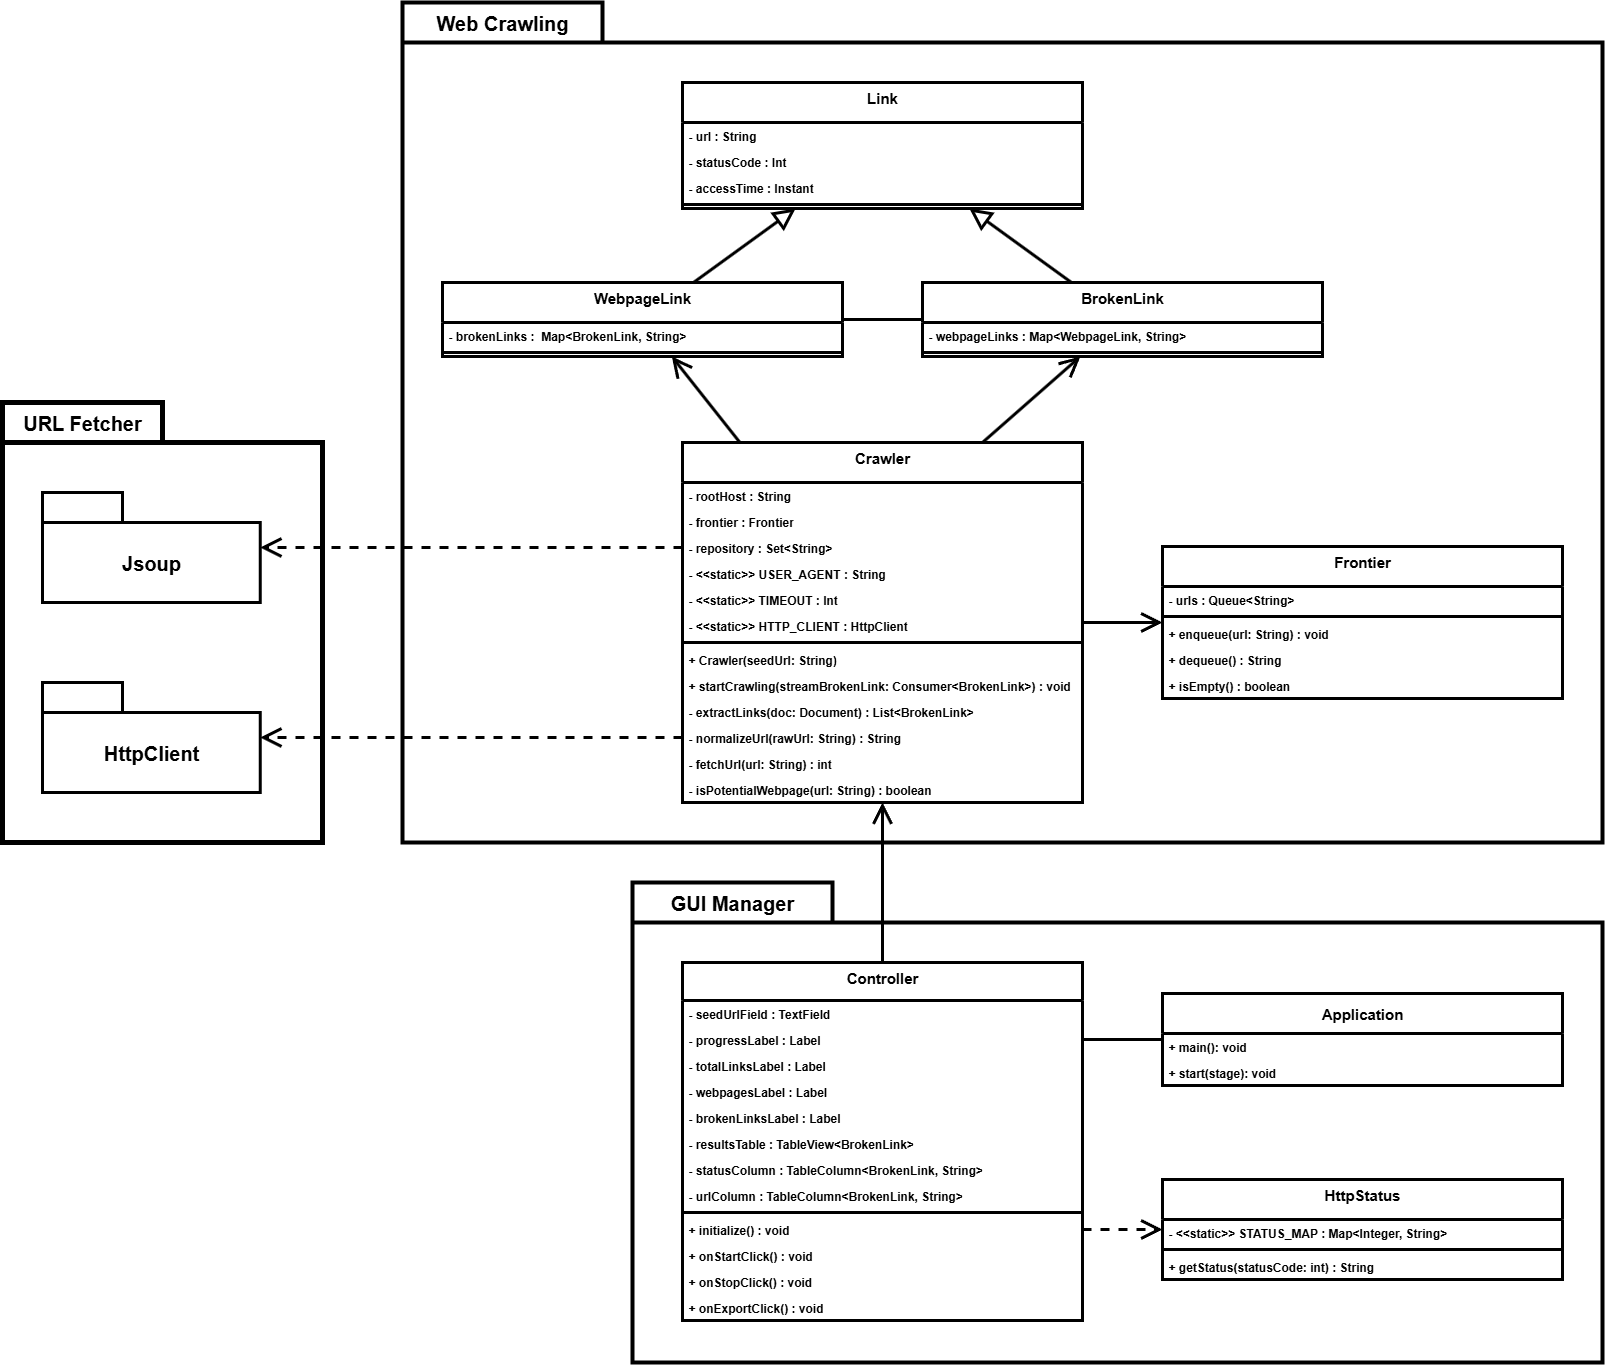
\includegraphics[width=0.95\textwidth]{Gambar/040100-class-diagram.png}
    \caption{Diagram kelas aplikasi}
    \label{fig:class-diagram}
\end{figure}


\section{Perancangan Alur}
\label{sec:04-perancangan-alur}

Perancangan alur menggambarkan interaksi antarobjek pada sistem \textit{Broken Link Checker} selama proses pemeriksaan tautan berlangsung. Interaksi ini divisualisasikan dalam bentuk \textit{sequence diagram} yang menunjukkan urutan pesan antarobjek sejak pengguna memulai pemeriksaan hingga proses selesai tanpa interupsi. Diagram lengkap ditunjukkan pada Gambar~\ref{fig:sequence-crawl}.

Berikut adalah penjelasan dari diagram pada Gambar~\ref{fig:sequence-crawl}:

\begin{enumerate}
    \item (1) Pengguna memasukkan \textit{seed URL} pada GUI.  
    \item (2) Pengguna menekan tombol \textit{Check}.  
    \item (3) GUI memanggil metode \texttt{onCheckClick()} pada \texttt{Controller}.  
    \item (4) \texttt{Controller} membuat objek \texttt{Crawler} baru.  
    \item (5) \texttt{Crawler} menambahkan URL awal ke \texttt{Frontier} melalui \texttt{enqueueUrl()}.  
    \item (6) \texttt{Controller} memanggil \texttt{startCrawling()} pada \texttt{Crawler}.  
    \item (7–8) \texttt{Crawler} masuk ke dalam \textit{loop} dengan mengambil URL dari \texttt{Frontier} menggunakan \texttt{dequeue()}, yang mengembalikan URL paling depan.  
    \item (9) URL di-\textit{fetch} oleh \texttt{Crawler}.  
    \item (10–12) Jika terjadi \texttt{error}, maka dibuat objek \texttt{BrokenLink}. Objek ini dikirim ke \texttt{Controller} melalui \texttt{streamBrokenLink()}, kemudian (12-13) ditampilkan pada tabel \textit{BrokenLink} di GUI.  
    \item (14–20) Jika status code hasil \texttt{fetch} oke, maka dilakukan:  
    \begin{enumerate}
        \item (14) Parsing HTML.  
        \item (15–16) Ekstraksi dan normalisasi URL dari dokumen.  
        \item (17) Dibuat objek \texttt{WebpageLink}.  
        \item (18–20) Objek ini dikirim ke \texttt{Controller} melalui \texttt{streamWebpageLink()} dan ditampilkan di tabel \textit{WebpageLink} pada GUI.  
    \end{enumerate}
    \item (21–26) Untuk setiap URL hasil ekstraksi (\textit{loop}):  
    \begin{enumerate}
        \item Jika URL adalah halaman web, maka dimasukkan kembali ke \texttt{Frontier} melalui \texttt{enqueueUrl()}.  
        \item Jika URL bukan halaman web, dilakukan \texttt{fetch}.  
        \item (23–26) Jika \texttt{fetch} error, dibuat objek \texttt{BrokenLink}, dikirim ke \texttt{Controller} (\texttt{streamBrokenLink()}), kemudian diperbarui pada tabel dan ditampilkan di GUI.  
    \end{enumerate}
    \item (27–29) Proses berulang sampai \texttt{Frontier} kosong. Pada akhir siklus, \texttt{Crawler} menghentikan proses, \texttt{Controller} menandai proses selesai, dan GUI menampilkan status akhir serta ringkasan hasil.  
\end{enumerate}

\begin{figure}[H]
    \centering
    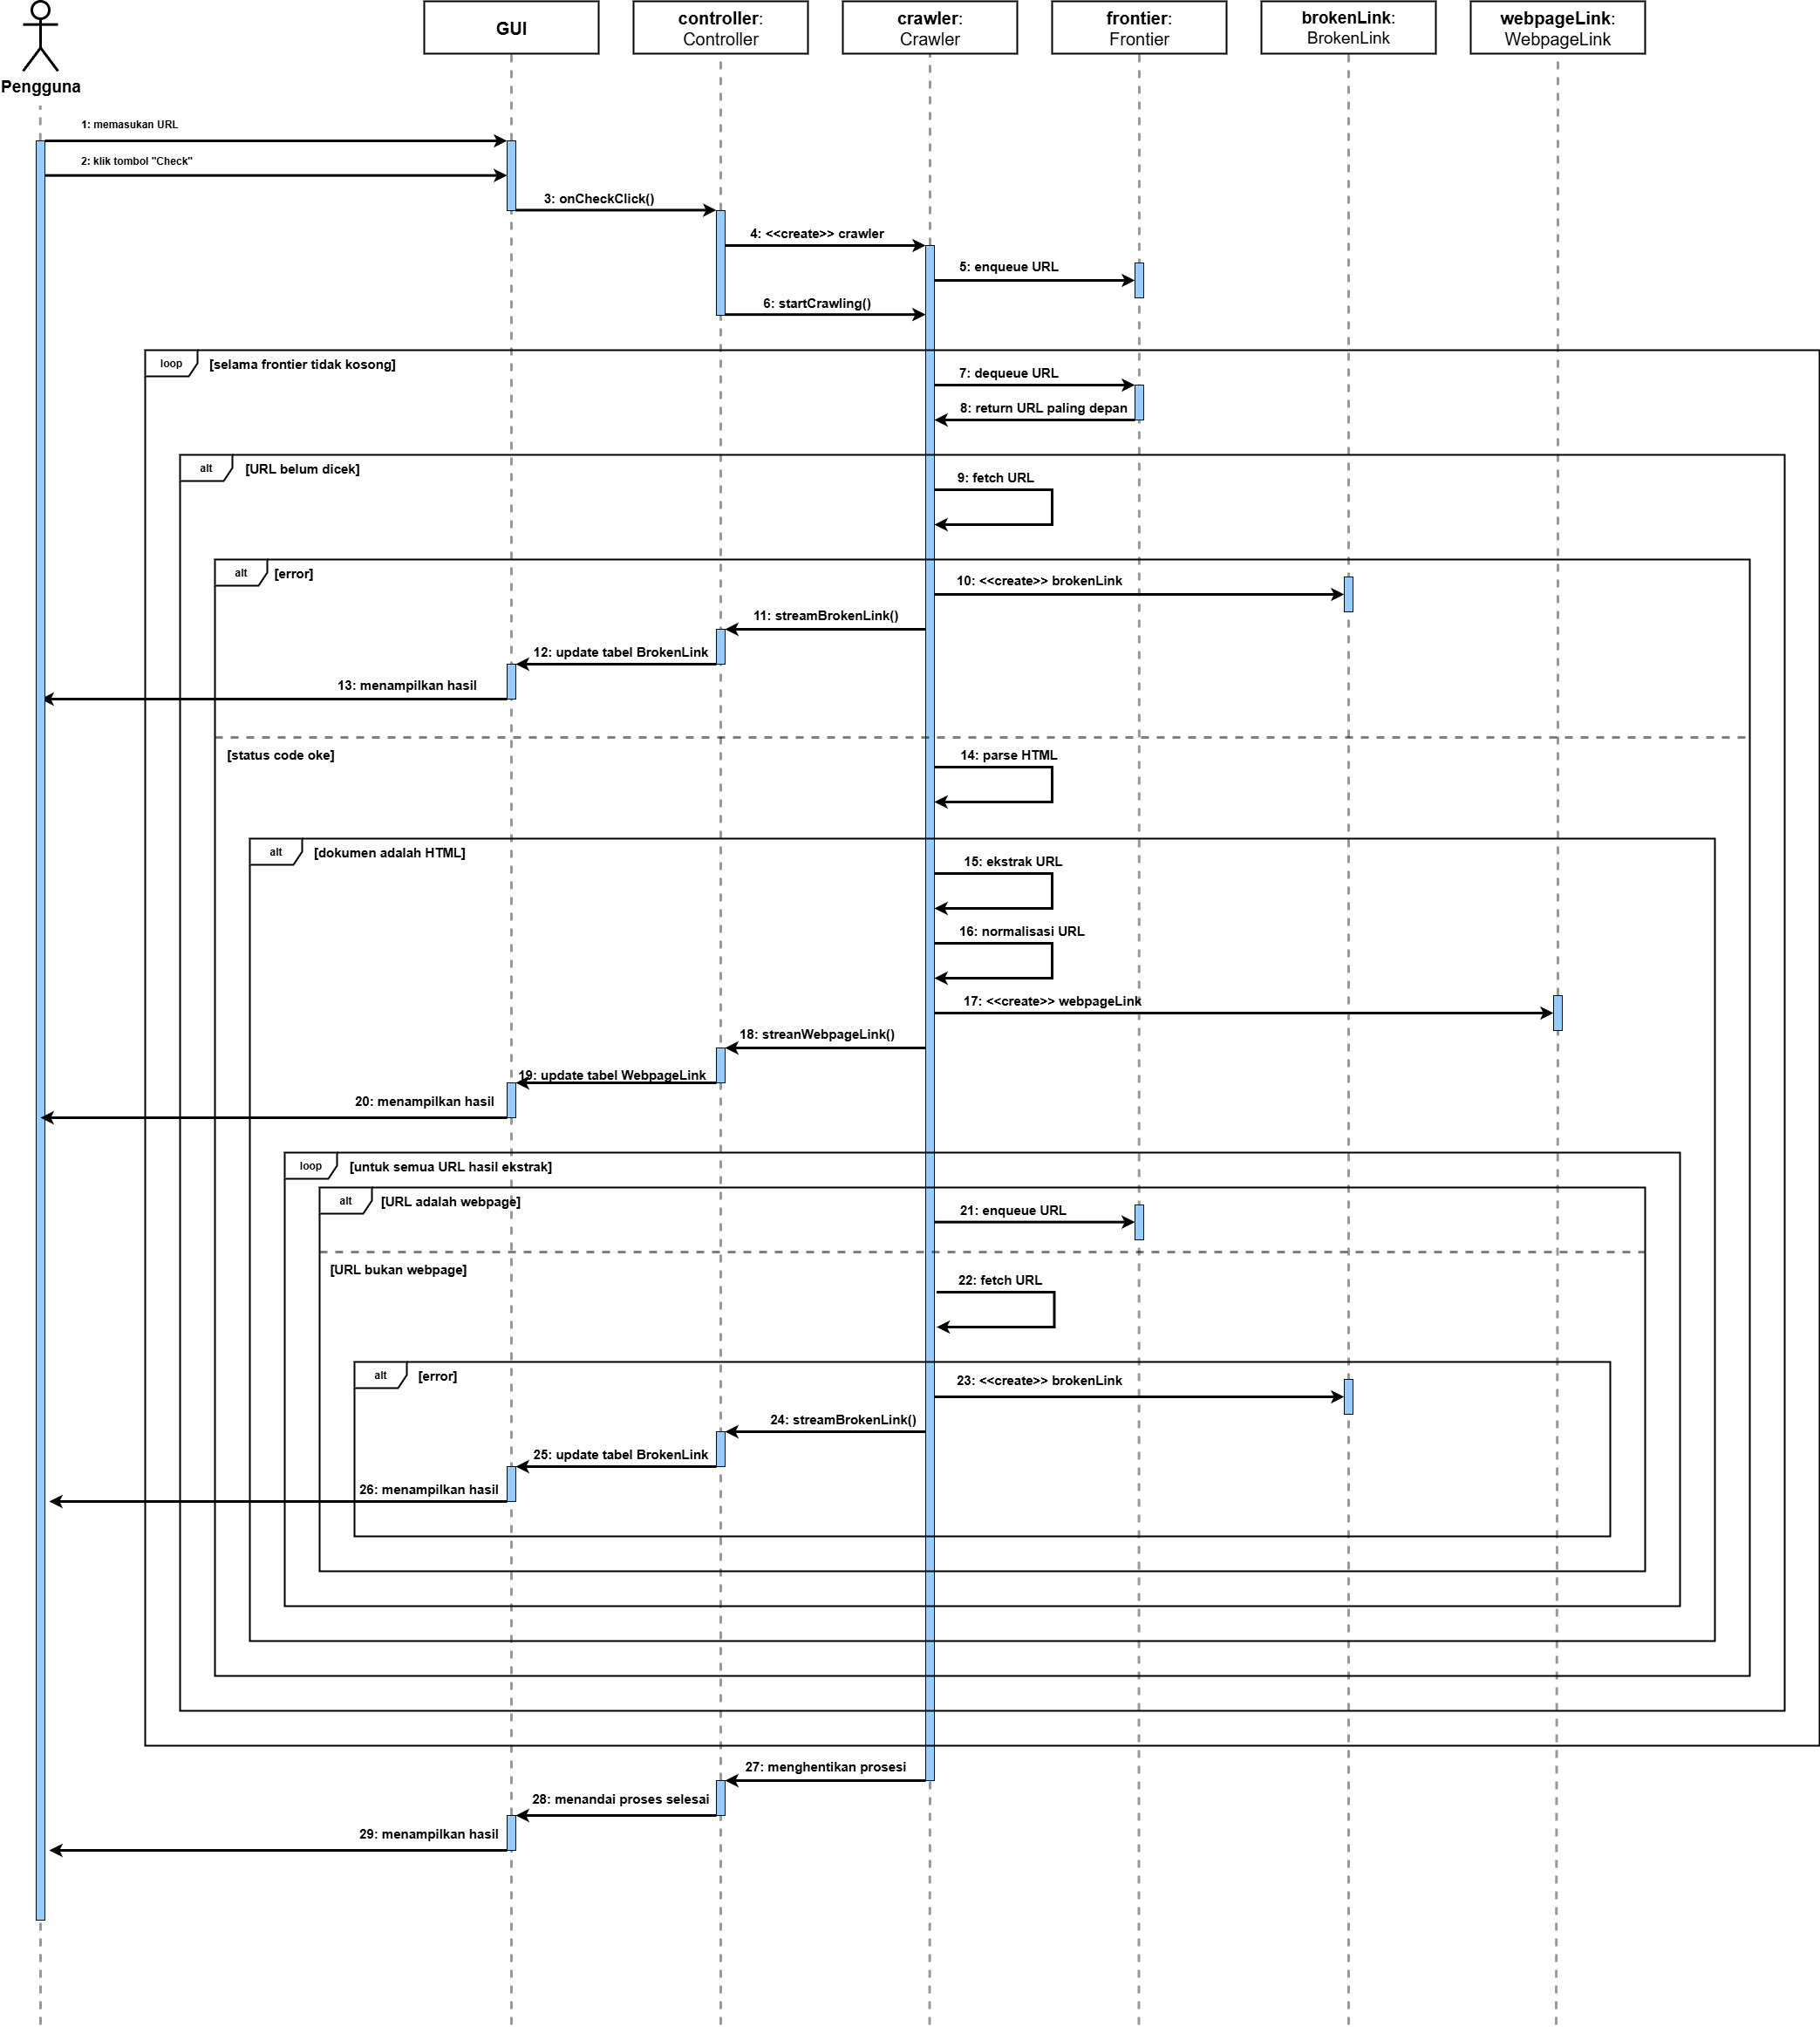
\includegraphics[width=1\textwidth]{Gambar/040200-sequence-diagram.png}
    \caption{Sequence diagram proses pemeriksaan tautan}
    \label{fig:sequence-crawl}
\end{figure}


\section{Perancangan Antarmuka}
\label{sec:04-perancangan-antarmuka}
Perancangan antarmuka pengguna dibuat dalam bentuk desain fidelitas tinggi dengan tujuan untuk memberikan gambaran visual yang mendekati tampilan akhir aplikasi berbasis JavaFX. Perancangan ini mempertimbangkan aspek keterbacaan, konsistensi elemen antarmuka, serta kemudahan interaksi bagi pengguna dalam menjalankan proses pemeriksaan tautan rusak.

\begin{enumerate}
    \item \textbf{Jendela Utama} \\
    Jendela utama merupakan tampilan awal yang muncul ketika aplikasi dijalankan. Halaman ini memfasilitasi pengguna untuk memasukkan URL situs web yang akan diperiksa, memulai atau menghentikan proses pemeriksaan, serta menampilkan hasil secara langsung. Elemen-elemen penting pada jendela ini ditunjukkan pada Gambar~\ref{fig:rancangan-jendela-utama} dan dijelaskan sebagai berikut:
    
    \begin{enumerate}
        
        \item \textbf{Kolom Masukan URL}: digunakan untuk memasukkan alamat situs web yang akan diperiksa.
        
        \item \textbf{Tombol Start}: digunakan untuk memulai proses pemeriksaan tautan.
        
        \item \textbf{Tombol Stop}: menghentikan proses pemeriksaan yang sedang berlangsung.
        
        \item \textbf{Checking Status}: menampilkan status terkini dari proses pemeriksaan, seperti \textit{Checking}, \textit{Stopped}, atau \textit{Completed}.
        
        \item \textbf{Total Links}: menunjukkan jumlah total tautan yang ditemukan selama proses \textit{crawling}.
        
        \item \textbf{Webpage Links}: menunjukkan jumlah tautan yang merupakan halaman situs web.
        
        \item \textbf{Broken Links}: menunjukkan jumlah tautan rusak yang ditemukan selama proses pemeriksaan.
        
        \item \textbf{Opsi Filter URL}: digunakan untuk menentukan jenis pencarian pada kolom URL. Opsi yang tersedia adalah:
        \begin{itemize}
            \item \textbf{Equals}: menampilkan hasil dengan URL yang sama persis.
            \item \textbf{Contains}: menampilkan hasil yang mengandung teks tertentu pada URL.
            \item \textbf{Starts With}: menampilkan hasil dengan URL yang diawali teks tertentu.
            \item \textbf{Ends With}: menampilkan hasil dengan URL yang diakhiri teks tertentu.
        \end{itemize}
        
        \item \textbf{Kolom Masukan Filter URL}: berfungsi untuk memasukkan kata kunci pencarian URL sesuai dengan opsi filter yang dipilih sebelumnya.
        
        \item \textbf{Opsi Filter Status Code}: digunakan untuk menyaring hasil berdasarkan kategori kode status HTTP. Opsi yang tersedia adalah:
        \begin{itemize}
            \item \textbf{Equals}: menampilkan tautan dengan kode status tertentu.
            \item \textbf{Greater Than}: menampilkan tautan dengan kode status lebih besar dari nilai yang dimasukkan.
            \item \textbf{Less Than}: menampilkan tautan dengan kode status lebih kecil dari nilai yang dimasukkan.
        \end{itemize}
        
        \item \textbf{Kolom Masukan Filter Status Code}: digunakan untuk memasukkan nilai numerik kode status HTTP sesuai dengan jenis filter yang dipilih pada poin sebelumnya.
        
        \item \textbf{Tombol Export}: digunakan untuk mengekspor hasil pemeriksaan ke dalam berkas Excel.
        
        \item \textbf{Tabel Hasil}: menampilkan daftar hasil pemeriksaan dalam bentuk tabel dengan dua kolom utama:
        \begin{enumerate}
            \item \textbf{Kolom Status}: menampilkan kode status HTTP dan \textit{reason phrase}.
            \item \textbf{Kolom URL}: menampilkan alamat tautan rusak.
        \end{enumerate}
        
        \item \textbf{Pagination}: digunakan untuk menavigasi hasil pemeriksaan jika jumlah tautan yang ditemukan cukup banyak.
    
    \end{enumerate}

    \begin{figure}[H]
        \centering
        \includegraphics[width=0.95\textwidth]{Gambar/040301-jendela-utama.png}
        \caption{Rancangan Halaman Utama}
        \label{fig:rancangan-jendela-utama}
    \end{figure}

    \item \textbf{Jendela Detail Broken Link} \\
    Jendela ini muncul ketika pengguna memilih salah satu tautan rusak pada tabel hasil. Elemen-elemen penting pada jendela ini ditunjukkan pada Gambar~\ref{fig:rancangan-jendela-detail-broken-link} dan dijelaskan sebagai berikut:
    
    \begin{enumerate}
        
        \item \textbf{Kolom URL}: menampilkan alamat lengkap dari tautan rusak yang sedang diperiksa.
        
        \item \textbf{Kolom Status}: menampilkan kode status HTTP dan \textit{reason phrase}.
        
        \item \textbf{Tabel Referensi Tautan}: berisi daftar halaman yang menjadi sumber dimana tautan rusak ditemukan, dengan dua kolom utama:
        \begin{enumerate}
            \item \textbf{Anchor Text}: teks tautan yang muncul pada halaman sumber.
            \item \textbf{Source Webpage}: URL halaman tempat tautan rusak ditemukan.
        \end{enumerate}
    \end{enumerate}

    \begin{figure}[H]
        \centering
        \includegraphics[width=0.95\textwidth]{Gambar/040302-jendela-detail-broken-link.png}
        \caption{Rancangan Jendela Detail Broken Link}
        \label{fig:rancangan-jendela-detail-broken-link}
    \end{figure}

\end{enumerate}

